\subsubsection{git简介}

git 是一个开源的分布式版本控制系统,用于敏捷高效地处理任何或小或大的项目,它可以在任何时间点,将文档的状态作为更新记录保存起来,也可以在任何时间点,将更新记录恢复回来。Git可以帮我们做到很多事情,比如代码的版本控制,分支管理,也提供了便于多人合作的平台。

在linux上安装git

\begin{tcode}
	sudo apt install git
\end{tcode}

\subsubsection{git基本概念}

在git中有一些比较重要的基本概念:

\textbf{本地仓库}:对本地代码进行管理的仓库,会包含代码的所有历史版本。

\textbf{远程仓库}:在开发者可以访问的网络内的某个服务器上有一个包含所有版本的仓库。

开发者可以把本地的新版本推送到远程仓库上,也可以把远程仓库上的新版本拉取到本地仓库上。由此可见,远程仓库为不同开发者之间的协作提供了一个渠道。

\textbf{工作区}:在本地计算机上的项目目录,你在这里进行文件的创建、修改和删除操作。工作区包含了当前项目的所有文件和子目录。

\textbf{暂存区}:临时存储区域,它包含了即将被提交到版本库中的文件快照。

\textbf{版本库}:包含项目的所有版本历史记录,每次提交都会在版本库中创建一个新的快照,这些快照是不可变的,确保了项目的完整历史记录。

\textbf{分支}:简单来说就是同一棵树上的两个分叉,实际上是指向更改快照的指针。

\textbf{暂存}:添加文件到暂存区准备提交。

\textbf{提交}:提交暂存区中的内容到本地仓库。

\textbf{推送}:推送本地仓库中的内容到远程仓库。

\textbf{克隆}:从远程仓库下载代码到本地的过程。

\textbf{合并}:假设分支A和分支B是从节点P分叉出来的,合并之后分支A和分支B会在一个新的节点后会和。

\textbf{变基}:从节点P开始,把分支A中各个节点按提交的顺序加在分支B的上面,因为一个节点对应一次内容改变,所以分支A中不想要的改变可以在变基的过程中跳过相应的节点。变基其实也可以理解成是另一种合并,只不过他的合并会让提交历史更为干净清晰。

\textbf{子模块}:将一个 git 仓库作为另一个 git 仓库的子目录。它能让你将另一个仓库克隆到自己的项目中,同时还保持提交的独立。

\subsubsection{git基本配置}

git 提供了一个叫做 git config 的命令,用来配置或读取相应的工作环境变量。这些环境变量,决定了 Git 在各个环节的具体工作方式和行为。这些变量可以存放在以下三个不同的地方:

\begin{enumerate}
\item /etc/gitconfig 文件:系统中对所有用户都普遍适用的配置。若使用 git config 时用 --system 选项,读写的就是这个文件。

\item \texttildelow /.gitconfig 文件:用户目录下的配置文件只适用于该用户。若使用 git config 时用 --global 选项,读写的就是这个文件。

\item 当前项目的 Git 目录中的配置文件(也就是工作目录中的 .git/config 文件):这里的配置仅仅针对当前项目有效。每一个级别的配置都会覆盖上层的相同配置,所以 .git/config 里的配置会覆盖 /etc/gitconfig 中的同名变量。
\end{enumerate}

\textbf{配置用户信息(个人访问令牌)}

github已经弃用了原先用个人用户名称和电子邮件地址来在每次提交代码时记录提交者的信息的方案,改用个人访问令牌。配置个人访问令牌的方法如下:

\begin{enumerate}
\item 在github设置界面点击进入“Developer settings”,访问 Personal Access Tokens中的Tokens(classic)页面
\item 点击 “Generate new token”,选择“Generate new token(classic)”
\item 为令牌选择一个描述性名称,选择 repo 权限,点击 “Generate token” 生成令牌,复制生成的令牌
\item 在提交代码时,当提示输入用户名和密码时,输入你的 GitHub 用户名和新生成的个人访问令牌即可
\end{enumerate}

\textbf{配置ssh密钥}

克隆github上的私人仓库不能使用https协议,只能使用SSH协议进行克隆,因此想要正常使用github还需要配置SSH密钥,具体方法如下:

\begin{enumerate}
\item 生成SSH密钥

\begin{tcode}
	ssh-keygen
\end{tcode}

生成后可在\texttildelow 目录下找到.ssh文件夹
\item 进入.ssh文件夹,复制其中id\_rsa.pub文件中的内容
\item 在github中进入个人设置界面,选择“SSH and GPG keys”,点击“New SSH key”
\item 给新的SSH起个标题,并将刚刚复制的内容粘贴到下方的文本框中,点击“Add SSH key”
\end{enumerate}

配置好后就可以克隆私人仓库中的代码了。

\subsubsection{git基本操作}

git的学问很多,各种操作也是五花八门,这里只列举出git工具的基本操作供读者参考。

\begin{center}  % 表格整体居中
\textbf{git基本操作}

	\begin{tabular}{cc}  % 内容左对齐
		\toprule[1.5pt]
		命令 & 作用\\
		\midrule[1pt]
		$  git\enspace config\enspace --list    $		&检查已有的配置信息\\
		$  git\enspace --version    $		&查看git版本(验证安装)\\
		$  git\enspace clone\enspace \textless url\textgreater  $		&将远程仓库克隆到本地\\
		$  git\enspace remote\enspace add\enspace origin\enspace \textless url\textgreater    $		&本地仓库链接远程仓库\\
		$  git\enspace add   $		&添加文件到暂存区\\
		$  git\enspace status   $		&查看仓库当前状态,显示变更\\
		$  git\enspace commit\enspace -m\enspace "description"   $		&提交到本地仓库并添加描述\\
		$  git\enspace reset\enspace [--soft | --mixed | --hard]\enspace [HEAD]   $		&回退某一次提交的版本\\
		$  git\enspace rm   $		&将文件从暂存区和工作区中删除\\
		$  git\enspace checkout\enspace \textless branchname\textgreater   $		&分支切换\\
		$  git\enspace log   $		&查看提交历史\\
		$  git\enspace diff   $		&查看工作区和暂存区之间的差异\\
		$  git\enspace diff\enspace --cached   $		&查看暂存区和最后一次提交的差异\\
		$  git\enspace remote   $		&列出当前仓库中已配置的远程仓库\\
		$  git\enspace remote\enspace rename\enspace \textless old\textgreater\enspace \textless new\textgreater   $		&将已配置的远程仓库重命名\\
		$  git\enspace remote\enspace show\enspace <remote\textgreater   $		&显示指定远程仓库的详细信息\\
		$  git\enspace fetch\enspace [remote]   $		&提取远程仓库中更新的数据\\
		$  git\enspace merge\enspace [remote]/[branch]  $		&将远程仓库的更新合并到当前分支\\
		$  git\enspace pull\enspace [remote]\enspace [branch]   $		&从远程获取代码并合并本地的版本\\
		$  git\enspace push\enspace \textless remote\textgreater\enspace <branch\textgreater :<remote\textgreater   $		&将本地版本上传到远程并合并\\
		$  git\enspace submodule\enspace init   $		&初始化子模块\\
		$  git\enspace submodule\enspace update   $		&更新子模块\\
		$  git\enspace submodule\enspace update\enspace --recursive\enspace --remote   $		&递归更新子模块并拉取最新更改\\
		$  git\enspace submodule\enspace add\enspace \textless url\textgreater\enspace [<path>]   $		&将Git仓库作为子模块加到当前仓库中\\
		\bottomrule[1.5pt]
	\end{tabular}
\end{center}
\begin{center}
	\textbf{git基本操作}
	
		\begin{tabular}{cc}
			\toprule[1.5pt]
			内容 & 作用\\
			\midrule[1pt]
			$  git\enspace submodule\enspace deinit\enspace [<path>]   $		&.git/config中移除子模块并删除文件\\
			$  git\enspace rm\enspace [<path>]   $		&子模块引用从仓库中删除并提交更改\\
			$  git\enspace submodule   $		&列出当前仓库中的所有子模块\\
			$  git\enspace branch   $		&查看所有分支\\
			$  git\enspace branch\enspace -r   $		&查看远程分支\\
			$  git\enspace branch\enspace -a   $		&查看所有本地和远程分支\\
			$  git\enspace merge\enspace \textless branch\textgreater   $		&将其他分支合并到当前分支\\
			$  git\enspace add\enspace \textless conflict-file\textgreater   $		&标记合并冲突解决完成\\
			$  git\enspace branch\enspace -b\enspace \textless branch\textgreater   $		&创建分支并更换到该分支\\
			$  git\enspace branch\enspace -d\enspace \textless branch\textgreater   $		&删除本地分支\\
			$  git\enspace branch\enspace -D\enspace <branch>$  		&强制删除未合并的分支\\
			$  git\enspace push\enspace origin\enspace --delete\enspace \textless branch\textgreater   $		&删除远程分支\\
			\bottomrule[1.5pt]
		\end{tabular}
	\end{center}

除了这些命令操作外,git中还有一个非常重要的工具\enspace——\enspace .gitignore忽略文件。尽管远程仓库在云端服务器上不会受到内存的限制,但是如果随便将大文件上传到远程仓库的话在下拉代码的时候会耗时非常久甚至拉代码失败。因此,上传至远程仓库中的内容一定是最核心的部分。

但是,在本地工作区往往会需要那些不需要被上传的“无用文件”,为了能在不上传“无用文件”的同时保证本地工作区的正常工作,我们就需要在本地工作区新建一个.gitignore文件,里面记录着不需要被版本库跟踪的文件,这样就能拥有一个干净简洁的版本库了。

需要注意的是,.gitignore只能忽略尚未提交到仓库的未被追踪的文件。如果一个文件已经被提交过了,此时再在.gitignore文件中添加忽略此文件时会发现这个文件依旧存在于版本库中。要想清除这个文件首先要将其从索引中删除:

\begin{tcode}
	git rm --cached .env
\end{tcode}

这条命令会从版本库中删除文件,但不删除实际的文件。这意味着该文件仍然在你的本地系统和工作目录中作为一个被忽略的文件存在。此时可以重新提交修改过的.gitignore文件来使新的忽略生效。

所以最好的方法还是在创建一个新的仓库的时候就把.gitignore文件写好,在首次提交前忽略不需要上传的文件。

.gitignore文件也有自己的语法,这里同样也列举一些用法:

\begin{center}
\textbf{.gitignore语法}

	\begin{tabular}{cc}
		\toprule[1.5pt]
		内容 & 作用\\
		\midrule[1pt]
		$  /text.txt    $		&忽略位于项目根目录下的 text.txt 文件\\
		$  /test/text.txt    $		&忽略位于项目根目录下test目录中的text.txt文件\\
		$  text.txt   $		&忽略任何 text.txt 文件\\
		$  test/   $		&忽略整个目录及其所有内容\\
		$  text   $		&忽略任何名字带有 test 的文件和目录\\
		$  img*   $		&忽略所有名称以 img 开头的文件和目录\\
		$  *.md   $		&忽略所有以 .md 文件扩展名结尾的文件\\
		$  !README.md   $		&不忽略 README.md 文件\\
		\bottomrule[1.5pt]
	\end{tabular}
\end{center}

\subsubsection{git工作流程}

git的基本工作流程就是从创建新仓库(或克隆别人的仓库),链接本地仓库和远程仓库或者建立新的分支(可选),修改完成后添加到暂存区,然后提交到本地,最后再推送回远程仓库的过程,可以参考下面这幅图。

\begin{figure}[H]
    \centering
    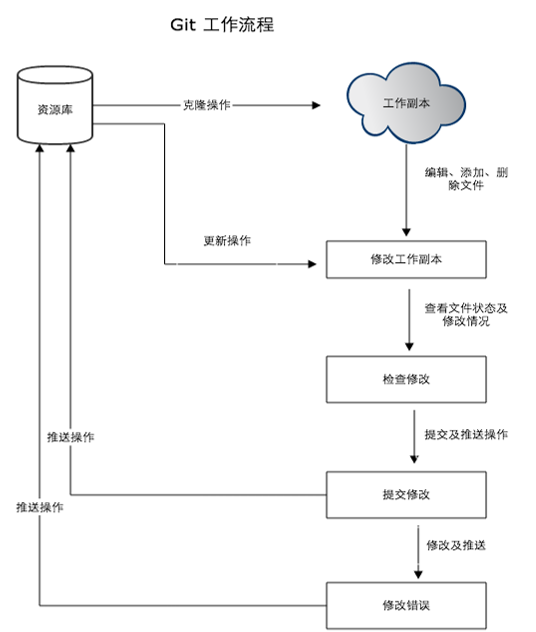
\includegraphics[width=0.7\textwidth]{git.png}
    \caption{git工作流程示意图} % 图片标题
    \label{fig:git} % 图片标签,用于引用
\end{figure}

对自己的仓库进行版本管理主要用到以下这些命令:

\begin{center}
\textbf{git工作流程基本命令}

	\begin{tabular}{c}
		\toprule[1.5pt]
		  git\enspace init       \\
		  git\enspace clone\enspace [url]    \\
		  git\enspace branch\enspace -b\enspace <branch>       \\
		  git\enspace remote\enspace add\enspace origin\enspace [url]       \\
		  git\enspace add       \\
		  git\enspace status       \\
		  git\enspace commit\enspace -m\enspace "description"       \\
		  git\enspace push\enspace <remote>\enspace <branch>:<remote>       \\
		  git\enspace pull\enspace [remote]\enspace [branch]       \\
		\bottomrule[1.5pt]
	\end{tabular}
\end{center}

使用git时我们可以选择直接在终端中通过命令行的方式提交代码,这种方式有时不够直观,因此除了命令行我们还可以使用一些git的图形化工具,比如GitKraken等等,当然也可以直接在clion或vscode中使用git相关插件,这些插件也提供了直观的版本库界面来辅助我们管理代码。

